\chapter{System implementation}
\section{Data collection}

\noindent
For the analysis of the websites, data had to be collected from the various websites. The data collected was mainly links contained in that website and presence of some rich files. Collection of this data could be done in two major ways:
\subsection{a) Use of search engines}

\noindent
Due to the vast number of websites and web pages, search engines are used as a starting point to navigating the World Wide Web. Search engines act as a gateway via which users surf the World
Wide Web. Thus, if a website appears in a search engine's results, it is visible to the public. Search engines have large databases with information about the websites. They crawl the websites and update their databases every so often. They provide a lot of information useful to webometrics and are vital in determining the visibility and impact of a university's website.

\noindent
In order for search engines to be used in the webometric process, they need to support programmatic searches and provision of results through facilities like APIs. This further limits the list of search engines that could be used in the process. Search engines that could be used in the data collection process are very few. They include: Google, Yahoo, Bing, Exalead, Ask, Alexa, Gigablast, Google Scholar, Live Academic.

\noindent
This limitation could be overcome by using the information they provide via web pages. Search engines provide web pages through which users can enter their search terms and submit to the engine. The engine searches its database and returns the results in a webpage to the user. This method is user-friendly but not program friendly. Even so, the information could be extracted from the result returned from the engine in a webpage programmatically.

\noindent
One major problem with search engines is their limited coverage of the World Wide Web. They cover just but the tip of the iceberg that is the World Wide Web. Some of the sites left out by search engines include websites requiring logging in or registration, unlinked  content and scripted content. Newly created sites are also not immediately available in search engine results.

\noindent
Search engines results are irregular and vary from one search engine to another. Different search engines produce different results for the same search term. This is majorly because the methods used to search and rank pages differ between the different search engines. Some factors may also be considered by the engine while computing its results. Such factors include location of the user, whether the user is logged in, preferred languages etc.

\noindent
Another problem with search engines is that they may not be up-to-date with the changes or updates made to websites. Search engines crawl websites after some time which may lead them to miss changes made to a website. Some of them may not have crawled the websites, thus not appear in the results. Broken links also pollute search engine results. Thus, the use of these results may lead to inaccurate findings.

\subsection{b) Use of web crawlers}
\noindent
A web crawler is a program that downloads web pages, extracts links from those pages. Web crawlers are designed to move from page to page in a website following links in the web pages. They are initially given one URL, usually the website’s top level page or home page. The web crawler downloads the page and extracts the links in the page. The extracted links could then be visited, links extracted from it and the process repeated. By repeating this process, the crawler could crawl the whole website.
A website could be thought of as a tree, with the root node being the start URL. The children of the root node are the web pages linked to the root node via links in the root node.

\begin{figure}[H]
	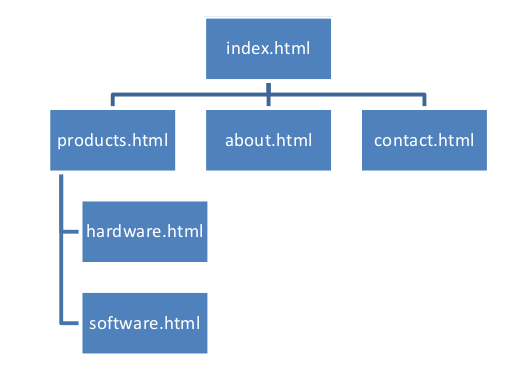
\includegraphics[width=\linewidth,scale=0.5]{../static/img/webtree.png}
	\caption{Sample website tree structure}
\end{figure}


\noindent
The web crawler starts at index.html, finds links to products.html, about.html and contact.html. The pages about.html and contact.html have no links in their pages thus are leaf nodes and no further action is taken. The page products.html has two links, hardware.html and software.html, which are followed. This process continues until the crawler reaches all the leaf nodes.

\noindent
Crawlers can be configured to target specific websites, web pages or elements in the website. They offer more credible results than search engines since:
\begin{enumerate}
\item They use the most recent website pages at the time of the crawl
\item There is a high probability that they will cover the whole domain
\item They can be tailored to look for specific information in websites.
\end{enumerate}

\subsubsection{Structure of a web crawler}

\noindent
A web crawler’s structure can vary from simple to very complex depending on the task it was created to accomplish. A simple web crawler could have two main parts, a page fetcher and a link extractor. The page fetcher is responsible for downloading web pages given a web page’s URL. The pages fetched are fed to the link extractor which extracts URLs from the pages. The extracted links are then fed to the page fetcher and the cycle continues. A simple web crawler could check for duplicate extracted URLs. Such a crawler, focused on URLs only, is a URL crawler. A more complex web crawler would do more than just extract links. For example, it would save pages to disk, extract keywords from pages, and check for duplicate page content, among other tasks. On top of URLs, these crawlers are also concerned with web page content. Such a crawler is a content crawler. Content crawlers are more preferred in link analysis.

\noindent
Web pages themselves are a challenge to parse easily. This is mainly due to them being written poorly because the website developers do not follow syntactic and semantic rules governing HTML. Over time, web browsers have become resilient against this and developed ways of overcoming this major flaw e.g. by restructuring the DOM before displaying the page. Content crawlers should also be resilient to this flaw to be able to parse content better.

\noindent
Traversing a website tree might bring up challenges. For example, if a page has a link referring to itself, the crawler might end up going into an infinite loop if it follows such a link. Also, links to the root node (start page) in the child nodes might also mean the crawler will traverse the website infinitely. A good example of this is navigation bars. They may contain the current page’s URL and the home page’s URL. One page could have multiple inlinks which would mean the crawler will visit a page more than one which is inefficient and resource consuming. Therefore such links should be filtered out. In some websites, different pages could have similar content. The crawler needs to filter this out also. Web pages A and B could be considered to be similar if:
\begin{enumerate}
\item a) They both have the same URL
\item b) They both have the same content
\item c) They both have almost similar content
\end{enumerate}

\noindent
Use of crawlers on a particular website requires its web server to serve pages faster than it was intended to do. Crawlers request for pages faster than people do via web browsers. This means the web server will use more resources than intended. If not regulated, it would mean the web crawler could cause a DOS on the server. Worse still, a distributed web crawler could cause a DDOS. Due to the possibilities of this, some web servers could deny service to bots. One simple way of identifying bots is by the time between requests. Bots have far shorter time between requests than humans. Thus regulation and throttling are required to control requests. Web technologies like javascript, flash and java are a hindrance to effective web crawling. These technologies allow developers to write links outside the standard format thus not all links in a website could be found. Links not in the format “<a href=’’></a>” are not considered. Javascript allows links to be dynamically generated or even written in a format not known to the crawler. Some links are stored in javascript files which are not looked at by the crawler. They give the users more freedom and control over what information they want to extract from websites. Nevertheless, crawlers require much more resources (time, money, computing resources, and human resources) to design and implement than using already existing search engines.

\subsubsection{Web crawler implementation}
The web crawler was implemented in Python programming language using a framework for web scraping called scrapy.
\begin{figure}[H]
	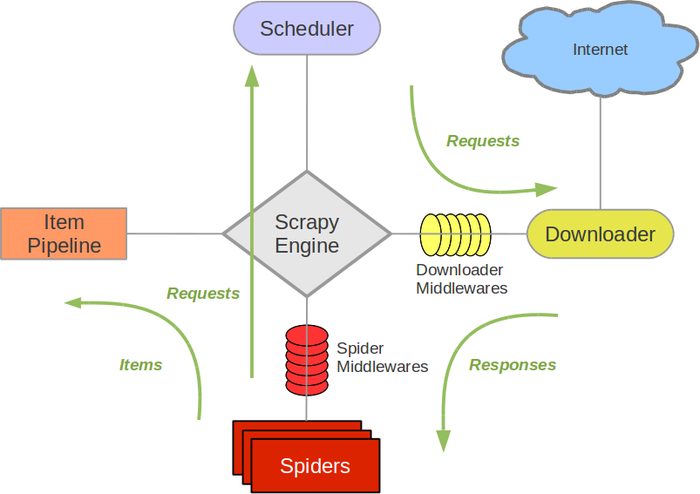
\includegraphics[width=\linewidth,scale=0.5]{../static/img/scrapy.png}
	\caption{Architecture of web crawler}
\end{figure}


\noindent
To avoid collection of duplicate links, three methods were employed. First, a list of visited URLs was kept and updated as pages are visited and downloaded. Before a page is visited, it is checked against the list of visited pages. If present in the list, it the page has been visited and the duplicate is dropped. If not, the link is visited and added to the list. The second method involved generating a hash for a web page's contents and comparing it to other web page's hashes that were captured earlier. A match between the new hash the stored hashes meant another page with the same content was already crawled and the new page discarded. By weeding out duplicate pages, duplicate URLs which would have been extracted are avoided. This method made it easy and fast to compare content from different web pages without comparing content value strings. However, this method was unable to discern between pages with almost similar content e.g. pages with only one character is different. The last method was to check the freshly extracted links against a list of the stored extracted links. Any newly extracted link found in the stored extracted links was dropped.

\subsubsection{Spider traps}
\subsubsection{Web crawler ethics}
\noindent
Crawlers can be configured to target specific websites, webpages or elements in the website. They offer more credible results than search engines since:
\begin{enumerate}
\item a) they use the most recent website pages at the time of the crawl
\item b) there is a high probability that they will cover the whole domain [[ please confirm this theory ]]
\item c) they can be tailored to look for specific information in websites.
\end{enumerate}
\noindent
They give the users more freedom and control over what information they want to extract from
websites. Nevertheless, crawlers require much more resources (time, money, compting resources,
human resources) to design and implement than using already existing search engines.
This project used both approaches to provide more information about the website being analysed.
The search engines were used for link analysis while the crawler was used to check within the
Kenyan academic webspace.

\noindent
The academic instututions chosen in this project were academic institutions recognized by the
ministry of education and had independent websites. Some institutions may not have dedicated
domains, some may have more than one and others may share their domain with other third
parties. Some institutions may have different domains for different units within themselves.

\subsubsection{Data storage}
\noindent
Data collected from the websites crawled had to be stored for future analysis. Storage was possible in two ways : 
\begin{enumerate}
\item \itemhead{Traditional relational databases}
\noindent
They provide the most common solution for storing data. They aim to provide data integrity even though this is done while compromising performance. The web crawler collects numerous pages per second on a good network connection. Therefore, the crawler generates alot of data in a short amount of time. This would lead to the system hitting the database with inserts multiple times per unit time and the RDBMS trying to validate and ensure data integrity. This would undoubtedly develop into a bottleneck for the system in terms of scalability and speed (especially write speed).

\item \itemhead{Flat files}
\noindent
They provide the simplest solution of the three choices. The format chosen to store the data was JSON. The data was stored as JSON lines not JSON objects. This was done to ensure the reading and writing of the files was done on a line by line basis not as one object to ensure minimal memory consumption and I/O access delays. The system at first used json files to store the data though it became evident that file location would become a thorny issue. 

\item \itemhead{NoSQL databases}
\noindent
They come in different forms e.g. document-oriented databases, graph databases, column-oriented databases, key-value datastores e.t.c. They were developed to overcome the constrictions of traditional SQL databases. When compared to relational databases, NoSQL databases are more scalable and provide superior performance, when it comes to large volumes of data. The system used a document-oriented database to store the crawled data. This was done so as to adapt to the already existing data format, JSON, which had been used before in flat files.
\end{enumerate}

\subsubsection{Web crawler server}
A web crawler server was used to manage web crawlers. It scheduled, paused, resumed and stopped crawls. It was autonomous from the rest of the system.

\noindent
The initial implementation of this was a generic server bundled with the web crawler framework. This implementation allowed crawls to be started, paused, resumed and stopped but could not schedule crawls. The implementation was also unable to cater for more than one crawl at a time. Each web crawling instance had its own server, thus it proved difficult to co-ordinate.

\noindent
The second attempt at the server was in form of a dedicated web crawler server called scrapyd. It is basically a scheduler to run web crawlers for one time jobs. It provided very useful functionalities e.g. viewing logs, managing running crawls and others. One major improvement over the first attempt was the fact that scrapyd could run multiple crawls simultaneously. However, control over the running of the web crawls proved to be too cumbersome. Pausing and resuming web crawls was not handled by the server while scheduling of the spiders for repeated runs was not efficient.

\noindent
The third attempt at the server was -----
\subsubsection{Message queues}
\noindent
A message queue was used to do computationally or time intensive tasks that should not impact the user's experience of the application.

\section{Data analysis}
Webometric formula
Visibility + Size + Rich files + Papers
50\% + 25\% + 12.5\% + 12.5\% = 100\%


\section{Data presentation}
This relied heavily on the input of the website administrator


\section{Resources}
The project used the following resources
Development environment
Software resources
Linux operating system, python programming language, apache \& nginx web servers, web browser
Hardware resources
Laptop Intel core i5 processor, over 4gb ram and over 2 gb free harddisk space
Internet connection
Production environment
Software resources
Hardware resources
Other resources



\section{Schedule}
\subsection{Project schedule}

\begin{table}[H]
\centering
\begin{tabular}{|p{0.5cm}|p{1.5cm}|p{1.5cm}|p{1.5cm}|p{1.5cm}|p{1.5cm}|p{1.5cm}|p{1.5cm}|p{2cm}|}
\hline
    \thead{Task No} & \thead{Task Name} & \thead{Planned Hours} & \thead{Actual Hours} & \thead{Planned Start Date} & \thead{Actual Start Date} &
    \thead{Planned End Date} & \thead{Actual End Date} & \thead{Deliverables}\\
\hline
    1 & Prepare proposal & & & & &  & Project proposal document\\
\hline
\hline
    2 & Desk study on website analysis & & & & &  & Research questions\\
\hline
\hline
    3 & Development of data gathering instruments & & & & &  & Formal and informal interview guides\\
\hline
\hline
    4 & Fieldwork : Interview & & & & & & Interview transcriptions\\
\hline
\hline
    5 & Data analysis and reporting & & & & & & Fieldwork report\\
\hline
\hline
    6 & Prepare proposal & & 22/10/2013 & & 25/10/2013 &  & Project proposal document\\
\hline
\hline
    7 & Prepare proposal & & 22/10/2013 & & 25/10/2013 &  & Project proposal document\\
\hline
\end{tabular}
\caption{Project schedule}
\end{table}

\subsection{Project Gantt chart}
\begin{figure}[H]
	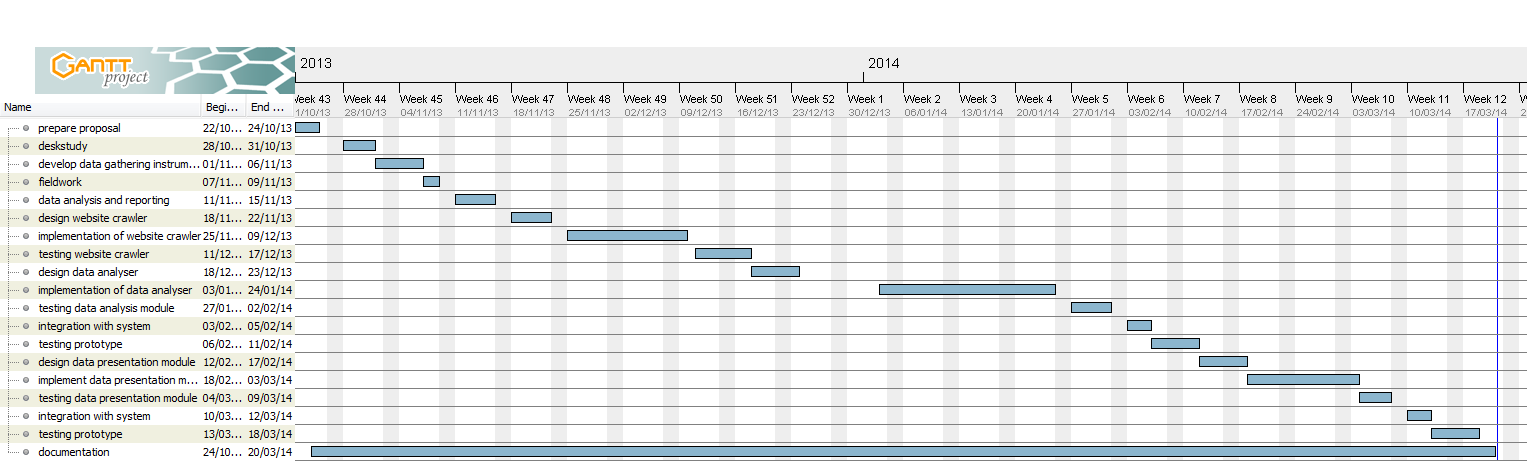
\includegraphics[width=\linewidth,scale=0.5]{../static/img/gantt.png}
	\caption{Architecture of web crawler}
\end{figure}





